% !TEX root = ../main.tex
\documentclass[../main.tex]{subfiles}


\begin{document}
\section{User authentication and authorization}

\subsection{Backed integration}

\subsubsection{Structure}

The code responsible for handling user authentication and authorization is located
under \texttt{src/auth} directory in the \textbf{backend} app directory.

\begin{figure}[H]
  \centering
  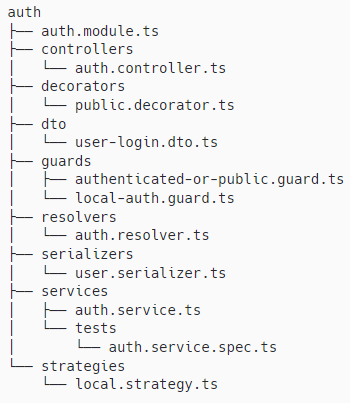
\includegraphics{file-tree/backend-auth-tree.png}
  \caption{Backend auth directory structure}
\end{figure}

The \texttt{auth} direcotry is furher divided into following subdirectories:
\begin{itemize}
  \item \texttt{controllers} - contains code which is responsible for handling incoming HTTP rquests and sending back responses (REST API)
  \item \texttt{decorators} - contains code that is used to extend other functions with additional functionality
  \item \texttt{dto} - contains data transfer objects, which define the data that is exchanged using REST API
  \item \texttt{guards} - contains code that is used to determinate if a given request should be authorized or not
  \item \texttt{resolvers} - contains GraphQL resolvers, which are used to handle incoming GraphQL requests
  \item \texttt{serializer} - contains code that is used to covert object to a representation that can be stored in cache
  \item \texttt{services} - contains classes that defined the business logic of the enclosing module, in this case the business logic is related to user authentication and authorization
\end{itemize}
This file structure is also used in other module of the backend application. It is a common practice to divide code into such subdirectories in NestJS applications.
To emphasize the role which each file plays an additional suffix is added to the file name. For example, \texttt{auth.controller.ts} is a controller file, \texttt{auth.service.ts} is a service file, etc.

In NestJS the application is build with modules, each module resides in its own directory under the \texttt{src} directory.
Modules have to defined what service is exposed to other modules and what is imported from other modules. In a special module class
which is often stored in a file suffixed with \texttt{.module.ts}. In this case the module class is defined in \texttt{auth.module.ts} file.

\begin{listing}[H]
  \tsfile{implementation/code/auth/auth.module.ts}
  \caption{Auth module class}
  \label{lst:auth-module}
\end{listing}

The module class is created using the \texttt{@Module} decorator imported from NestJS library.
The purpose of fileds of the module class decorator are as follows:
\begin{itemize}
  \item \textbf{imports} - defines what other modules are imported into the current module
  \item \textbf{providers} - contain list of services, resolvers and guards that are provided by the current module for the apllication
  \item \textbf{controllers} - defines what controllers are provided by the current module
  \item \textbf{exports} - defines what services, resolvers and guards are exported from the current module and can be used by other modules
\end{itemize}

\subsubsection{Passport.js integration}

Passport.js is a library that handles the authentication logic in the application.
To intgrate passport into the application first a startegy has to be defined. In this case the \texttt{LocalStrategy} is used.
This startegy performs using the username and password provided by the user. The logic of the startegy is defined in \texttt{local.strategy.ts} file.

\begin{listing}[H]
  \tsfile{implementation/code/auth/local.strategy.ts}
  \caption{Local strategy implementation}
\end{listing}

In this application the \textbf{email} field will be used as the username. For Passport to be able to properly parse the login DTO the
\texttt{usernameField} property has to be set to \texttt{email}. The \texttt{validate} method is used to validate the user credentials.

The defined strategy is then used to define an \texttt{AuthGuard} which will perform the authentication logic and reject the request if the user
did not pass the authentication credentials (username and password for the \texttt{LocalStrategy}).

\begin{listing}[H]
  \tsfile{implementation/code/auth/local.strategy.ts}
  \caption{Local strategy guard}
\end{listing}

This guard is then used to decorate a controller method.

\begin{listing}[H]
  \tsfile{implementation/code/auth/local-guard-usage.ts}
  \caption{Local strategy guard usage example}
  \label{code:local-guard-usage}
\end{listing}

Posting a request to the \texttt{/login} endpoint will first invoke the \texttt{LocalAuthGuard}.
This guard will inspect the request object for user credentials and if they are not present it will reject the request.
If the credentials are present the \texttt{validate} method of \texttt{LocalAuthGuard} will be invoked and the validation suceeds then request will be authorized, and the
\texttt{login} method will be invoked. Otherwise, the request will be rejected and the \texttt{UnauthorizedException} will be thrown.

To complete the authentication the result of the \texttt{login} method has to be serialized and stored in the session.
To later deserialize the session middleware has to be registered in the application.

\begin{listing}[H]
  \tsfile{implementation/code/auth/express-session.middleware.ts}
  \caption{Express session middleware}
\end{listing}

The express middleware will write and retive the session data from the Redis cache and store it in the \texttt{req.session} object.
A session cookie will be sent to the client and the client will send it back with each request. The session cookie will be used to identify the session.
The data that is stored in the session is provided by the passport middleware.

\begin{figure}[H]
  \centering
  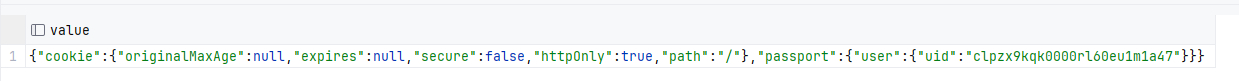
\includegraphics[width=\textwidth]{auth/redis-data.png}
  \caption{Session data stored in Redis}
\end{figure}


\begin{listing}[H]
  \tsfile{implementation/code/auth/passport.middleware.ts}
  \caption{Passport session middleware}
\end{listing}



\end{document}